\documentclass[12pt,a4paper,oneside]{book}

\usepackage[utf8]{inputenc}
\usepackage[T1]{fontenc}
\usepackage{lmodern}
\usepackage{graphicx}
\usepackage{amsmath,amssymb}
\usepackage{geometry}
\usepackage{hyperref}
\usepackage{xcolor}
\usepackage{listings}
\usepackage{microtype}
\usepackage{booktabs}
\usepackage{caption}
\usepackage{tikz}
\usetikzlibrary{arrows.meta, positioning, fit, backgrounds, calc, shapes.geometric}

\geometry{margin=1in}
\emergencystretch=1.5em

\makeatletter
\newcommand{\chapterauthor}[1]{%
  {\parindent0pt\vspace*{-15pt}%
  \linespread{1.1}\large\itshape\begin{flushright}#1\end{flushright}%
  \par\nobreak\vspace*{25pt}}
  \@afterheading%
}
\makeatother

% =====================================================================
% Syntax Highlighting Configuration for C++
% =====================================================================
\definecolor{codeblue}{rgb}{0.0, 0.2, 0.75}
\definecolor{codegreen}{rgb}{0.13, 0.55, 0.13}
\definecolor{codegray}{rgb}{0.42, 0.42, 0.42}
\definecolor{codepurple}{rgb}{0.55, 0.0, 0.75}
\definecolor{backcolour}{rgb}{0.97, 0.98, 0.99}

\lstdefinestyle{cppstyle}{
    backgroundcolor=\color{backcolour},   
    commentstyle=\color{codegreen}\itshape,
    keywordstyle=\color{codeblue}\bfseries,
    numberstyle=\tiny\color{codegray},
    stringstyle=\color{codepurple},
    basicstyle=\ttfamily\footnotesize,
    breakatwhitespace=false,         
    breaklines=true,                 
    captionpos=b,                    
    keepspaces=true,                 
    numbers=left,                    
    numbersep=6pt,                  
    showspaces=false,                
    showstringspaces=false,
    showtabs=false,                  
    tabsize=2,
    frame=lines,
    rulecolor=\color{black!25}
}
\lstset{style=cppstyle}

\hypersetup{
    colorlinks=true,
    linkcolor=blue!70!black,
    citecolor=blue!70!black,
    urlcolor=blue!70!black
}

\begin{document}

\mainmatter

% =====================================================================
% C++ OOP Mini-Project Chapter Template
% Save this file as: ProjectNumber_ShortName.tex (e.g., 03_SQL_Engine.tex)
% =====================================================================

\chapter[Audio Synthesizer (WAV Generator)]{Audio Synthesizer (WAV Generator): Algorithmic Sound Synthesis and RIFF/WAVE Binary Serialization}
\chaptermark{Audio Synthesizer (WAV Generator)}
\markboth{CHAPTER \thechapter. AUDIO SYNTHESIZER (WAV GENERATOR)}{CHAPTER \thechapter. AUDIO SYNTHESIZER (WAV GENERATOR)}
\chapterauthor{Shailesh (251150), Sirthik (251153)}

% =====================================================================
% 1. INTRODUCTION AND PROBLEM STATEMENT
% =====================================================================
\section{Introduction and Problem Statement}
Sound synthesis represents the mathematical intersection of physics, digital signal processing (DSP), and computer systems engineering. In an era where audio generation is often abstracted away behind monolithic third-party multimedia frameworks (such as SDL, PortAudio, or OpenAL), understanding the low-level generation of acoustic pressure waves from mathematical primitives provides fundamental insights into memory efficiency, real-time algorithms, and low-level binary data serialization.

The primary objective of this project is to architect and implement an extensible, decoupled, and highly performant \textbf{Audio Synthesizer and WAV Generator} in modern C++ (C++17). The system is engineered from the ground up without relying on external multimedia runtimes for audio generation or file formatting. Instead, the application directly generates discrete periodic waveforms, modulates their amplitude across temporal domains using an Attack-Decay-Sustain-Release (ADSR) envelope generator, and formats the synthesized raw pulse-code modulation (PCM) audio samples into a standard Microsoft Resource Interchange File Format (RIFF) WAVE audio file via unbuffered binary C++ file streams (\texttt{std::ofstream}).

The engineering requirements stipulated for the project comprise:
\begin{enumerate}
    \item \textbf{Waveform Generation:} Mathematically generate three fundamental periodic acoustic waveforms: pure sinusoidal waves (\textit{Sine}), odd-harmonic rich pulses (\textit{Square}), and full harmonic-spectrum ramps (\textit{Sawtooth}).
    \item \textbf{Object-Oriented Architecture:} Implement an abstract base class \texttt{Oscillator} defining a pure virtual polymorphic interface for dynamic sample generation, alongside dedicated derived classes implementing concrete mathematical transfer functions.
    \item \textbf{Temporal Dynamic Envelope:} Implement an encapsulated \texttt{Envelope} class providing four-stage piecewise linear ADSR modulation to prevent acoustic clicking artifacts caused by instantaneous step transients.
    \item \textbf{Raw Binary Serialization:} Assemble canonical 44-byte RIFF/WAVE file headers and serialize 16-bit signed integer little-endian audio samples into persistent storage using formatted binary C++ file streams (\texttt{std::ofstream}).
    \item \textbf{Defensive Validation:} Guard against acoustic aliasing by strictly enforcing the Nyquist-Shannon sampling theorem limit ($0 < f < f_s / 2$) and clamping peak amplitude values to prevent integer overflow.
    \item \textbf{Dual Frontend Interaction:} Deliver both a scriptable Command-Line Interface (CLI) supporting parameterized flags and an interactive Terminal User Interface (TUI) powered by FTXUI featuring real-time oscilloscopic waveform previews.
\end{enumerate}

From an end-user perspective, the system provides sound designers, audio researchers, and students with an intuitive utility capable of generating calibrated acoustic test signals, musical tones, and customized synthesis sweeps exported directly into high-fidelity uncompressed 16-bit PCM \texttt{.wav} files compatible with any industry-standard media player (VLC, Windows Media Player) or digital audio workstation (DAW such as Audacity, Ableton Live, or FL Studio).

% =====================================================================
% 2. SCOPE AND FEATURE SET
% =====================================================================
\section{Scope and Feature Set}
The project delivers an end-to-end audio rendering pipeline partitioned into a static synthesis library (\texttt{synth\_core}) and frontend driver executables. The feature set includes:

\begin{itemize}
    \item \textbf{Feature 1 (Multi-Waveform Timbre Generation):} Full algorithmic synthesis of three fundamental wave profiles:
    \begin{itemize}
        \item \textit{Sine Wave:} Pure fundamental frequency ($f$) devoid of harmonic overtones; provides a smooth, mellow, acoustic tuning-fork response ($x(n) = \sin(2\pi \phi_n)$).
        \item \textit{Square Wave:} Composed exclusively of odd integer harmonics ($f, 3f, 5f, \dots$) decaying at $1/n$ amplitude; delivers a hollow, resonant retro-gaming timbre ($x(n) = \text{sgn}(\sin(2\pi \phi_n))$).
        \item \textit{Sawtooth Wave:} Composed of both even and odd harmonics ($f, 2f, 3f, \dots$) decaying at $1/n$; delivers a bright, buzzy, aggressive timbre ideal for synth leads ($x(n) = 2\phi_n - 1$).
    \end{itemize}

    \item \textbf{Feature 2 (Continuous Normalized Phase Accumulation):} A normalized phase accumulator $\phi \in [0.0, 1.0)$ updated as $\phi_{n+1} = (\phi_n + f / f_s) \pmod{1.0}$, maintaining sample-accurate phase tracking across arbitrary sampling frequencies ($f_s$) and eliminating phase tearing and frequency drift over extended durations.

    \item \textbf{Feature 3 (Piecewise Linear ADSR Dynamic Envelope):} A 4-stage time-domain amplitude modulator:
    \begin{itemize}
        \item \textit{Attack ($T_A$):} Linear ramp from zero amplitude to maximum unity gain ($1.0$).
        \item \textit{Decay ($T_D$):} Linear ramp down from peak amplitude to the configured sustain level.
        \item \textit{Sustain ($S$):} Maintained steady-state amplitude plateau ($S \in [0.0, 1.0]$).
        \item \textit{Release ($T_R$):} Linear decay from sustain down to absolute silence ($0.0$) prior to note termination.
    \end{itemize}

    \item \textbf{Feature 4 (Direct RIFF/WAVE Binary Stream Serialization):} Direct byte-level Little-Endian bit encoding and memory packing for the standard 44-byte canonical WAV header without reliance on external struct padding quirks. Supports arbitrary durations, configurable sampling rates (8\,kHz to 192\,kHz), and 16-bit signed integer quantizations.

    \item \textbf{Feature 5 (Defensive Boundary Validation and Nyquist Safety):} Enforces the Nyquist-Shannon sampling limit ($0 < f < f_s / 2$) to eliminate digital aliasing, clamps amplitude values to $[-1.0, 1.0]$ to prevent clipping, and validates non-negative envelope timing parameters.

    \item \textbf{Feature 6 (Dual Presentation Frontends):}
    \begin{itemize}
        \item \textit{CLI Executable (\texttt{synth}):} Optimized for rapid shell scripting, automated batch processing, and CI pipelines via standard flags (\texttt{--wave}, \texttt{--freq}, \texttt{--duration}, \texttt{--amp}, \texttt{--attack}, etc.).
        \item \textit{Interactive TUI (\texttt{synth-tui}):} Interactive terminal dashboard built using FTXUI featuring real-time Braille-canvas oscilloscopic waveform previews, dynamic ADSR envelope graphs, and parameter sliders.
    \end{itemize}
\end{itemize}

% ---------------------------------------------------------------------
% 2.1 TECHNOLOGY STACK
% ---------------------------------------------------------------------
\subsection{Technology Stack}
The system is engineered from the ground up utilizing modern, standardized technologies designed to achieve high computational throughput, platform independence, deterministic memory management, and zero third-party runtime dependencies for core signal synthesis. Table~\ref{tab:tech_stack} provides a comprehensive overview of the technologies, tools, and libraries utilized across the engineering lifecycle.

\begin{table}[htbp]
\centering
\caption{Comprehensive Technology Stack of the Audio-WAV-Synthesizer Project}
\label{tab:tech_stack}
\scriptsize
\begin{tabular}{@{}llllp{6.6cm}@{}}
\toprule
\textbf{Layer / Domain} & \textbf{Technology / Library} & \textbf{Standard / Version} & \textbf{License} & \textbf{Role and Architectural Rationale} \\ \midrule
\textbf{Primary Language} & Modern C++ & ISO/IEC C++17 & Open ISO & Deterministic memory management (RAII), zero-overhead abstractions, compile-time type safety, and direct byte-level binary streaming. \\
\textbf{DSP \& Core Logic} & C++ Standard Library & C++17 STL & ISO & \texttt{<memory>} (smart pointers), \texttt{<vector>} (contiguous sample buffers), \texttt{<cmath>} (trigonometrics), \texttt{<algorithm>} (\texttt{std::clamp}), \texttt{<cstdint>} (fixed-width integer types). \\
\textbf{Binary File I/O} & \texttt{std::ofstream} & C++ Standard Stream & ISO & Unbuffered raw binary file output with manual little-endian byte serialization, avoiding compiler struct padding quirks. \\
\textbf{Build Automation} & CMake & Version 3.14+ & BSD 3-Clause & Declarative target-based build orchestration; partitions the engine into a static library (\texttt{synth\_core}) and dual frontend binaries. \\
\textbf{TUI Interface} & FTXUI & Version 5.0.0 & MIT & Declarative functional terminal UI providing interactive parameter sliders, responsive layout, and keyboard-driven controls. \\
\textbf{Waveform Preview} & \texttt{ftxui::Canvas} & FTXUI Component & MIT & High-resolution oscilloscopic visualizer rendering continuous waveforms and ADSR curves using Unicode Braille dot matrices. \\
\textbf{Dependency Fetch} & CMake \texttt{FetchContent} & CMake Built-in & BSD 3-Clause & Automated remote fetching and hermetic building of external dependencies directly from GitHub repositories during configuration. \\
\textbf{Audio Format} & Microsoft RIFF/WAVE & Canonical 1991 Spec & Open Spec & Uncompressed 16-bit linear PCM audio container with 44-byte standard header, ensuring universal playback across all DAWs and OS players. \\
\textbf{Compiler Support} & GCC, Clang, MSVC & Modern Toolchains & Various & Cross-platform compilation enforcing rigorous compiler diagnostics (\texttt{-Wall -Wextra}) and platform-independent little-endian bit shifting. \\
\textbf{Verification Tools} & Audacity \& Hex Dumps & v3.x / Native CLI & GPL v2 / OS & Fast Fourier Transform (FFT) spectrum analysis, acoustic envelope inspection, and byte-level hexadecimal verification of WAV headers. \\
\bottomrule
\end{tabular}
\end{table}

The technical justification for each principal component of the technology stack comprises:
\begin{enumerate}
    \item \textbf{C++17 for Deterministic Real-Time DSP:} Digital sound synthesis requires continuous, jitter-free sample computation. High-level garbage-collected runtimes (e.g., Java, Python, or JavaScript) introduce non-deterministic stop-the-world pauses that can compromise real-time audio streams. C++17 was selected for its zero-cost abstraction guarantees, compile-time polymorphic safety, and deterministic Resource Acquisition Is Initialization (RAII) memory semantics via \texttt{std::unique\_ptr}.
    \item \textbf{Decoupled Modular Build via CMake 3.14+:} The project establishes a modular CMake architecture that isolates the core DSP algorithms into a standalone static library (\texttt{synth\_core}). This static library is compiled with strict warning diagnostics (\texttt{-Wall -Wextra}) and linked independently into both the lightweight CLI executable (\texttt{synth}) and the terminal UI executable (\texttt{synth-tui}).
    \item \textbf{Reactive Terminal Interface via FTXUI:} To provide visual feedback without the runtime overhead of heavy graphical toolkits (such as Qt or wxWidgets), the project leverages Arthur Sonzogni's FTXUI library. FTXUI provides a functional reactive component model and utilizes Unicode Braille characters ($2 \times 4$ dot matrix per glyph cell) through \texttt{ftxui::Canvas}, delivering high-resolution oscilloscope displays directly within standard terminal windows.
    \item \textbf{Zero-Runtime RIFF/WAVE Binary Serialization:} By directly assembling the 44-byte canonical RIFF/WAVE header and packing 16-bit little-endian integer samples via raw bit-shifting into \texttt{std::ofstream}, the system eliminates runtime dependencies on heavy third-party audio abstraction libraries (such as SDL2, PortAudio, or libsndfile). This guarantees complete architectural transparency, negligible binary footprint, and instant execution.
\end{enumerate}

% =====================================================================
% 3. OBJECT-ORIENTED ARCHITECTURE
% =====================================================================
\section{Object-Oriented Architecture}
The software architecture adheres rigorously to established Object-Oriented Programming (OOP) principles, guaranteeing high cohesion, loose coupling, and strict separation of concerns across audio synthesis, data modulation, and binary persistence.

\begin{enumerate}
    \item \textbf{Data Abstraction:} 
    The abstract base class \texttt{Oscillator} establishes a formal contract for periodic acoustic signal generators. Callers interact exclusively with the pure virtual member function \texttt{nextSample()}, abstracting away underlying trigonometric evaluations, phase increments, and piecewise boundary calculations.
    
    Listing~\ref{lst:oscillator_h} defines the abstract base interface. The virtual destructor ensures safe polymorphic deletion, and the phase advancement logic is declared \texttt{protected} to prevent external state tampering while remaining accessible to derived classes.

\begin{lstlisting}[language=C++, caption={Abstract Oscillator Base Class (\texttt{include/Oscillator.h})}, label={lst:oscillator_h}]
#pragma once

class Oscillator {
public:
    Oscillator(double frequency, double sampleRate);
    virtual ~Oscillator() = default; // Essential virtual destructor for polymorphism

    // Pure virtual method: must be realized by concrete waveform classes
    virtual double nextSample() = 0;

    void setFrequency(double frequency);
    void reset();

protected:
    void advancePhase();

    double frequency_;
    double sampleRate_;
    double phase_ = 0.0; // Normalized phase tracking [0.0, 1.0)
};
\end{lstlisting}

    \item \textbf{Polymorphism and Dynamic Dispatch:} 
    The core synthesis pipeline in \texttt{render()} operates uniformly on an abstract base pointer \texttt{std::unique\_ptr<Oscillator>}. At runtime, virtual method tables (vtables) resolve invocations of \texttt{nextSample()} to the appropriate concrete waveform realization (\texttt{SineOscillator}, \texttt{SquareOscillator}, or \texttt{SawtoothOscillator}) selected by the user via a Factory Method pattern, as shown in Listing~\ref{lst:synth_cpp}.

\begin{lstlisting}[language=C++, caption={Polymorphic Factory and Rendering Pipeline (\texttt{src/Synth.cpp})}, label={lst:synth_cpp}]
#include "SynthSettings.h"
#include "Envelope.h"
#include "Waveforms.h"
#include <memory>
#include <vector>

// Factory Pattern: Instantiates derived classes through abstract base pointer
static std::unique_ptr<Oscillator> makeOscillator(const SynthSettings& s) {
    switch (s.waveform) {
        case Waveform::Square:
            return std::make_unique<SquareOscillator>(s.frequency, s.sampleRate);
        case Waveform::Sawtooth:
            return std::make_unique<SawtoothOscillator>(s.frequency, s.sampleRate);
        case Waveform::Sine:
        default:
            return std::make_unique<SineOscillator>(s.frequency, s.sampleRate);
    }
}

std::vector<double> render(const SynthSettings& s) {
    const std::size_t total = static_cast<std::size_t>(s.duration * s.sampleRate);
    std::unique_ptr<Oscillator> osc = makeOscillator(s);
    Envelope env(s.attack, s.decay, s.sustain, s.release, s.sampleRate);

    std::vector<double> samples;
    samples.reserve(total);

    for (std::size_t i = 0; i < total; ++i) {
        // Polymorphic dynamic dispatch: osc->nextSample()
        const double wave = osc->nextSample();
        const double gain = env.amplitudeAt(i, total);
        samples.push_back(wave * gain * s.amplitude);
    }
    return samples;
}
\end{lstlisting}

    \item \textbf{Encapsulation and Information Hiding:} 
    Internal state attributes—such as the accumulated phase \texttt{phase\_}, frequency \texttt{frequency\_}, and envelope parameters (\texttt{attack\_}, \texttt{decay\_}, \texttt{sustain\_}, \texttt{release\_})—are strictly encapsulated with \texttt{private} or \texttt{protected} access specifiers. State mutations occur solely through validated constructors and controlled member functions, preventing corrupt out-of-order state transitions. Listing~\ref{lst:envelope_cpp} illustrates the encapsulated ADSR implementation.

\begin{lstlisting}[language=C++, caption={Encapsulated ADSR Dynamic Envelope Modulator (\texttt{src/Envelope.cpp})}, label={lst:envelope_cpp}]
#include "Envelope.h"
#include <algorithm>

Envelope::Envelope(double attack, double decay, double sustain, double release,
                   double sampleRate)
    : attack_(attack), decay_(decay), sustain_(sustain), release_(release),
      sampleRate_(sampleRate) {}

double Envelope::amplitudeAt(std::size_t sampleIndex,
                             std::size_t totalSamples) const {
    const double t = static_cast<double>(sampleIndex) / sampleRate_;
    const double length = static_cast<double>(totalSamples) / sampleRate_;

    double gain;
    if (attack_ > 0.0 && t < attack_) {
        gain = t / attack_; // 1. Attack: Linear ramp up [0.0 -> 1.0]
    } else if (decay_ > 0.0 && t < attack_ + decay_) {
        // 2. Decay: Linear ramp down [1.0 -> sustain]
        gain = 1.0 - (1.0 - sustain_) * ((t - attack_) / decay_);
    } else {
        gain = sustain_;    // 3. Sustain: Steady-state plateau
    }

    // 4. Release: Smooth fade-out to zero at note termination
    if (release_ > 0.0) {
        gain *= std::clamp((length - t) / release_, 0.0, 1.0);
    }
    return gain;
}
\end{lstlisting}

    \item \textbf{Inheritance and Code Reusability:} 
    The derived oscillator classes publicly inherit from \texttt{Oscillator}, directly reusing the underlying phase accumulator and sample-rate infrastructure while supplying distinct mathematical transfer functions, as shown in Listing~\ref{lst:waveforms_cpp}.

\begin{lstlisting}[language=C++, caption={Concrete Derived Waveform Implementations (\texttt{src/Waveforms.cpp})}, label={lst:waveforms_cpp}]
#include "Waveforms.h"
#include <cmath>

namespace {
constexpr double kTwoPi = 6.283185307179586476925286766559;
}

// 1. Pure Sine: Smooth trigonometric projection
double SineOscillator::nextSample() {
    const double sample = std::sin(kTwoPi * phase_);
    advancePhase();
    return sample;
}

// 2. Square Wave: Binary bipolar thresholding
double SquareOscillator::nextSample() {
    const double sample = (phase_ < 0.5) ? 1.0 : -1.0;
    advancePhase();
    return sample;
}

// 3. Sawtooth Wave: Linear bi-directional ramp
double SawtoothOscillator::nextSample() {
    const double sample = 2.0 * phase_ - 1.0;
    advancePhase();
    return sample;
}
\end{lstlisting}

    \item \textbf{Separation of Concerns (SoC):} 
    The system isolates mathematical sound generation (\texttt{Oscillator}), amplitude modulation (\texttt{Envelope}), configuration parameters (\texttt{SynthSettings}), low-level binary serialization (\texttt{WavWriter}), and presentation frontends (\texttt{main.cpp}, \texttt{tui.cpp}) into decoupled compilation units, ensuring that modifications to the storage format or UI do not impact the core DSP algorithms.
\end{enumerate}

% =====================================================================
% 3.1 CLASS DESIGN AND ASSOCIATIONS
% =====================================================================
\subsection{Class Design and Associations}
The relationships between the primary architectural components are structured as follows:
\begin{itemize}
    \item \textbf{Generalization (Inheritance):} \texttt{SineOscillator}, \texttt{SquareOscillator}, and \texttt{SawtoothOscillator} publicly inherit from the abstract base class \texttt{Oscillator}, realizing the pure virtual interface \texttt{nextSample()}.
    \item \textbf{Composition:} The rendering pipeline (\texttt{render()}) instantiates and manages the lifecycle of an \texttt{Oscillator} (via \texttt{std::unique\_ptr}) and an \texttt{Envelope} instance for the duration of the audio synthesis task.
    \item \textbf{Aggregation / Association:} The \texttt{SynthSettings} Plain Old Data (POD) structure aggregates configuration values alongside the strongly typed enumeration \texttt{Waveform}, decoupling parameter storage from processing logic.
    \item \textbf{Dependency:} The static utility class \texttt{WavWriter} depends upon normalized \texttt{std::vector<double>} sample buffers produced by \texttt{render()} and interacts directly with \texttt{std::ofstream} binary sinks.
\end{itemize}

% ---------------------------------------------------------------------
% UML CLASS DIAGRAM (NATIVE TIKZ)
% ---------------------------------------------------------------------
\begin{figure}[htbp]
\centering
\resizebox{0.95\textwidth}{!}{%
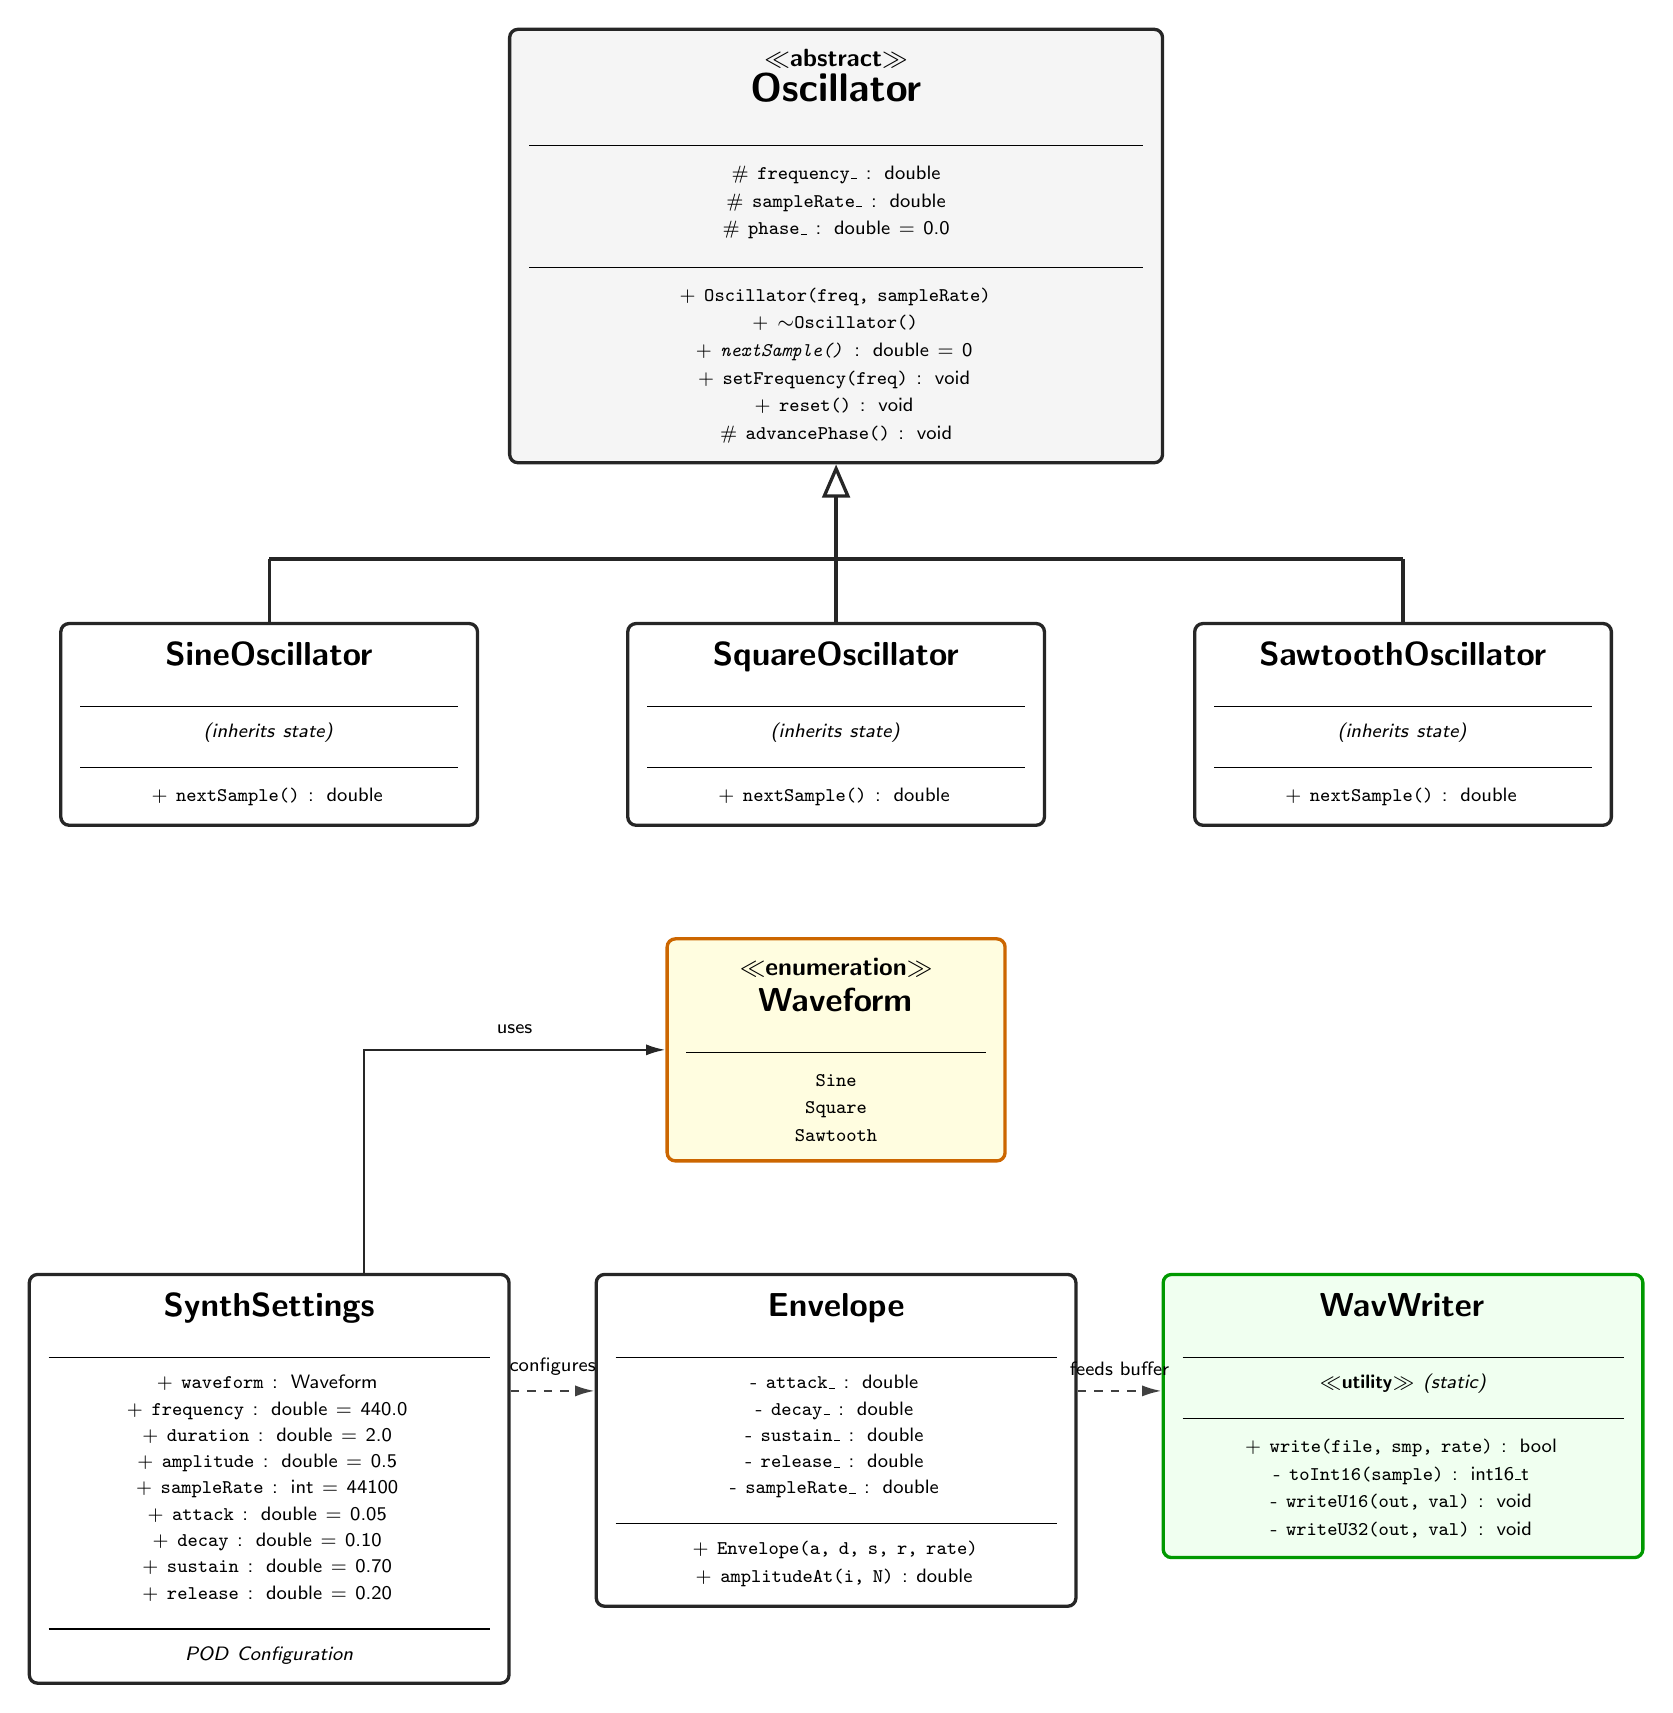
\begin{tikzpicture}[
    font=\small\sffamily,
    umlClass/.style={
        draw=black!85,
        very thick,
        fill=white,
        rounded corners=3pt,
        inner sep=7pt,
        align=left
    },
    umlAbstract/.style={
        umlClass,
        fill=gray!8
    },
    umlEnum/.style={
        umlClass,
        fill=yellow!12,
        draw=orange!80!black
    },
    umlWriter/.style={
        umlClass,
        fill=green!6,
        draw=green!60!black
    },
    depend/.style={
        -{Latex[length=7pt, width=4pt]},
        dashed,
        thick,
        draw=black!75
    },
    assoc/.style={
        -{Latex[length=7pt, width=4pt]},
        thick,
        draw=black!85
    }
]

    % =========================================================================
    % 1. TOP ROW: Abstract Base Class (Oscillator)
    % =========================================================================
    \node[umlAbstract, text width=7.8cm, anchor=north] (oscillator) at (0, 0) {
        \centering $\ll$\textbf{abstract}$\gg$\\[2pt]
        \centering\textbf{\Large Oscillator}\\[5pt]
        \rule{\linewidth}{0.5pt}\\[4pt]
        \scriptsize
        \# \texttt{frequency\_} : double\\[2pt]
        \# \texttt{sampleRate\_} : double\\[2pt]
        \# \texttt{phase\_} : double = 0.0\\[4pt]
        \rule{\linewidth}{0.5pt}\\[4pt]
        \scriptsize
        + \texttt{Oscillator(freq, sampleRate)}\\[2pt]
        + \texttt{$\sim$Oscillator()}\\[2pt]
        + \texttt{\textit{nextSample()}} : double = 0\\[2pt]
        + \texttt{setFrequency(freq)} : void\\[2pt]
        + \texttt{reset()} : void\\[2pt]
        \# \texttt{advancePhase()} : void\\[2pt]
    };

    % =========================================================================
    % 2. INHERITANCE BUS BAR (Guaranteed 1.2 cm below Oscillator bottom)
    % =========================================================================
    \coordinate (bus) at ([yshift=-1.2cm]oscillator.south);
    \coordinate (stemLeft) at (-7.2, 0 |- bus);
    \coordinate (stemCenter) at (bus);
    \coordinate (stemRight) at (7.2, 0 |- bus);

    % Upward arrow to Oscillator bottom with open UML triangle
    \draw[very thick, draw=black!85, -{Triangle[open, length=12pt, width=10pt]}] (stemCenter) -- (oscillator.south);

    % Horizontal distribution bus bar
    \draw[very thick, draw=black!85] (stemLeft) -- (stemRight);

    % =========================================================================
    % 3. SECOND ROW: Concrete Waveform Oscillators (0.8 cm below bus bar)
    % =========================================================================
    \node[umlClass, text width=4.8cm, anchor=north] (sineOsc) at ([yshift=-0.8cm]stemLeft) {
        \centering\textbf{\large SineOscillator}\\[4pt]
        \rule{\linewidth}{0.5pt}\\[3pt]
        \centering\scriptsize\textit{(inherits state)}\\[3pt]
        \rule{\linewidth}{0.5pt}\\[4pt]
        \centering\scriptsize + \texttt{nextSample()} : double\\[2pt]
    };

    \node[umlClass, text width=4.8cm, anchor=north] (squareOsc) at ([yshift=-0.8cm]stemCenter) {
        \centering\textbf{\large SquareOscillator}\\[4pt]
        \rule{\linewidth}{0.5pt}\\[3pt]
        \centering\scriptsize\textit{(inherits state)}\\[3pt]
        \rule{\linewidth}{0.5pt}\\[4pt]
        \centering\scriptsize + \texttt{nextSample()} : double\\[2pt]
    };

    \node[umlClass, text width=4.8cm, anchor=north] (sawOsc) at ([yshift=-0.8cm]stemRight) {
        \centering\textbf{\large SawtoothOscillator}\\[4pt]
        \rule{\linewidth}{0.5pt}\\[3pt]
        \centering\scriptsize\textit{(inherits state)}\\[3pt]
        \rule{\linewidth}{0.5pt}\\[4pt]
        \centering\scriptsize + \texttt{nextSample()} : double\\[2pt]
    };

    % Drop stems connecting bus bar to derived oscillators
    \draw[very thick, draw=black!85] (stemLeft) -- (sineOsc.north);
    \draw[very thick, draw=black!85] (stemCenter) -- (squareOsc.north);
    \draw[very thick, draw=black!85] (stemRight) -- (sawOsc.north);

    % =========================================================================
    % 4. THIRD ROW: Waveform Enumeration (1.4 cm below SquareOscillator)
    % =========================================================================
    \node[umlEnum, text width=3.8cm, anchor=north] (waveformEnum) at ([yshift=-1.4cm]squareOsc.south) {
        \centering $\ll$\textbf{enumeration}$\gg$\\[2pt]
        \centering\textbf{\large Waveform}\\[4pt]
        \rule{\linewidth}{0.5pt}\\[4pt]
        \centering\scriptsize
        \texttt{Sine}\\[2pt]
        \texttt{Square}\\[2pt]
        \texttt{Sawtooth}\\[2pt]
    };

    % =========================================================================
    % 5. FOURTH ROW: SynthSettings, Envelope, and WavWriter
    % =========================================================================
    \node[umlClass, text width=5.6cm, anchor=north] (envelope) at ([yshift=-1.4cm]waveformEnum.south) {
        \centering\textbf{\large Envelope}\\[4pt]
        \rule{\linewidth}{0.5pt}\\[3pt]
        \scriptsize
        - \texttt{attack\_} : double\\[1.5pt]
        - \texttt{decay\_} : double\\[1.5pt]
        - \texttt{sustain\_} : double\\[1.5pt]
        - \texttt{release\_} : double\\[1.5pt]
        - \texttt{sampleRate\_} : double\\[3pt]
        \rule{\linewidth}{0.5pt}\\[3pt]
        \scriptsize
        + \texttt{Envelope(a, d, s, r, rate)}\\[2pt]
        + \texttt{amplitudeAt(i, N)} : double\\[2pt]
    };

    \node[umlClass, text width=5.6cm, anchor=north] (settings) at (envelope.north -| stemLeft) {
        \centering\textbf{\large SynthSettings}\\[4pt]
        \rule{\linewidth}{0.5pt}\\[3pt]
        \scriptsize
        + \texttt{waveform} : Waveform\\[1.5pt]
        + \texttt{frequency} : double = 440.0\\[1.5pt]
        + \texttt{duration} : double = 2.0\\[1.5pt]
        + \texttt{amplitude} : double = 0.5\\[1.5pt]
        + \texttt{sampleRate} : int = 44100\\[1.5pt]
        + \texttt{attack} : double = 0.05\\[1.5pt]
        + \texttt{decay} : double = 0.10\\[1.5pt]
        + \texttt{sustain} : double = 0.70\\[1.5pt]
        + \texttt{release} : double = 0.20\\[3pt]
        \rule{\linewidth}{0.5pt}\\[3pt]
        \centering\scriptsize\textit{POD Configuration}\\[2pt]
    };

    \node[umlWriter, text width=5.6cm, anchor=north] (wavWriter) at (envelope.north -| stemRight) {
        \centering\textbf{\large WavWriter}\\[4pt]
        \rule{\linewidth}{0.5pt}\\[3pt]
        \centering\scriptsize $\ll$\textbf{utility}$\gg$ \textit{(static)}\\[3pt]
        \rule{\linewidth}{0.5pt}\\[4pt]
        \scriptsize
        + \texttt{write(file, smp, rate)} : bool\\[2pt]
        - \texttt{toInt16(sample)} : int16\_t\\[2pt]
        - \texttt{writeU16(out, val)} : void\\[2pt]
        - \texttt{writeU32(out, val)} : void\\[2pt]
    };

    % =========================================================================
    % 6. ASSOCIATIONS & DEPENDENCIES (Zero overlaps, clean routes)
    % =========================================================================
    % SynthSettings uses Waveform: orthogonal path up from settings.north then right to waveformEnum.west
    \draw[assoc] ([xshift=1.2cm]settings.north) |- node[near end, above=2pt, font=\scriptsize\sffamily] {uses} (waveformEnum.west);

    % SynthSettings configures Envelope: straight horizontal dashed arrow across generous gap
    \draw[depend] ([yshift=-1.5cm]settings.north east) -- node[midway, above=2pt, font=\scriptsize\sffamily] {configures} ([yshift=-1.5cm]envelope.north west);

    % Envelope feeds buffer to WavWriter: straight horizontal dashed arrow across generous gap
    \draw[depend] ([yshift=-1.5cm]envelope.north east) -- node[midway, above=2pt, font=\scriptsize\sffamily] {feeds buffer} ([yshift=-1.5cm]wavWriter.north west);

\end{tikzpicture}
}
\caption{UML Class Diagram: Depicts the polymorphic base interface \texttt{Oscillator}, derived concrete waveforms, configuration encapsulation via \texttt{SynthSettings}, temporal envelope shaping, and static binary serialization.}
\label{fig:uml_class}
\end{figure}

% ---------------------------------------------------------------------
% UML SEQUENCE DIAGRAM (NATIVE TIKZ)
% ---------------------------------------------------------------------
Figure~\ref{fig:uml_sequence} details the dynamic execution flow and message passing during synthesis:

\begin{figure}[htbp]
\centering
\resizebox{0.95\textwidth}{!}{%
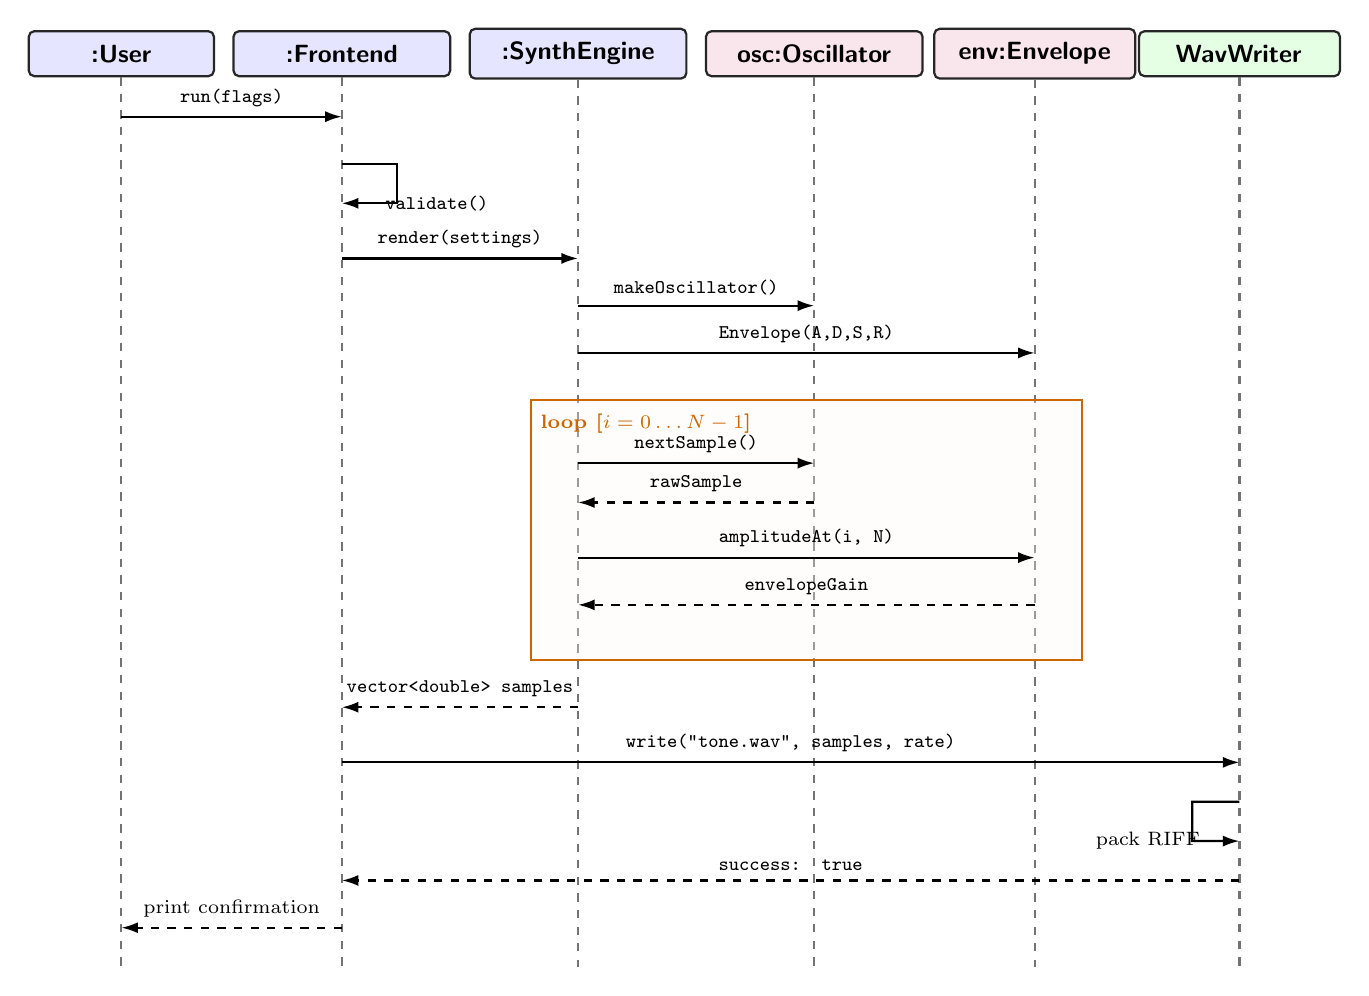
\begin{tikzpicture}[
    font=\small\sffamily,
    lifeline/.style={
        draw=black!55,
        thick,
        dashed
    },
    entity/.style={
        draw=black!85,
        thick,
        fill=blue!10,
        rounded corners=2pt,
        inner sep=5pt,
        align=center
    },
    msg/.style={
        thick,
        -{Latex[length=6pt, width=4pt]}
    },
    retMsg/.style={
        thick,
        dashed,
        -{Latex[length=6pt, width=4pt]}
    }
]

    % Lifeline Headers
    \node[entity, text width=2.0cm] (user)  at (0, 0)     {\textbf{:User}};
    \node[entity, text width=2.4cm] (cli)   at (2.8, 0)   {\textbf{:Frontend}};
    \node[entity, text width=2.4cm] (synth) at (5.8, 0)   {\textbf{:SynthEngine}};
    \node[entity, fill=purple!10, text width=2.4cm] (osc) at (8.8, 0) {\textbf{osc:Oscillator}};
    \node[entity, fill=purple!10, text width=2.2cm] (env) at (11.6, 0) {\textbf{env:Envelope}};
    \node[entity, fill=green!10, text width=2.2cm] (writer) at (14.2, 0) {\textbf{WavWriter}};

    % Vertical Lifelines
    \draw[lifeline] (user.south)   -- (0, -11.6);
    \draw[lifeline] (cli.south)    -- (2.8, -11.6);
    \draw[lifeline] (synth.south)  -- (5.8, -11.6);
    \draw[lifeline] (osc.south)    -- (8.8, -11.6);
    \draw[lifeline] (env.south)    -- (11.6, -11.6);
    \draw[lifeline] (writer.south) -- (14.2, -11.6);

    % Execution Steps
    \draw[msg] (0, -0.8) -- node[above, font=\scriptsize] {\texttt{run(flags)}} (2.8, -0.8);
    \draw[msg] (2.8, -1.4) -- ++(0.7, 0) -- ++(0, -0.5) -- node[right=2pt, font=\scriptsize] {\texttt{validate()}} (2.8, -1.9);
    \draw[msg] (2.8, -2.6) -- node[above, font=\scriptsize] {\texttt{render(settings)}} (5.8, -2.6);

    % Factory & Envelope Construction
    \draw[msg] (5.8, -3.2) -- node[above, font=\scriptsize] {\texttt{makeOscillator()}} (8.8, -3.2);
    \draw[msg] (5.8, -3.8) -- node[above, font=\scriptsize] {\texttt{Envelope(A,D,S,R)}} (11.6, -3.8);

    % Sample Loop Container
    \draw[thick, draw=orange!80!black, fill=orange!4, fill opacity=0.3] (5.2, -4.4) rectangle (12.2, -7.7);
    \node[anchor=north west, font=\bfseries\scriptsize, text=orange!80!black] at (5.2, -4.45) {loop [$i = 0 \dots N - 1$]};

    \draw[msg] (5.8, -5.2) -- node[above, font=\scriptsize] {\texttt{nextSample()}} (8.8, -5.2);
    \draw[retMsg] (8.8, -5.7) -- node[above, font=\scriptsize] {\texttt{rawSample}} (5.8, -5.7);
    \draw[msg] (5.8, -6.4) -- node[above, font=\scriptsize] {\texttt{amplitudeAt(i, N)}} (11.6, -6.4);
    \draw[retMsg] (11.6, -7.0) -- node[above, font=\scriptsize] {\texttt{envelopeGain}} (5.8, -7.0);

    % Return Buffer and Serialization
    \draw[retMsg] (5.8, -8.3) -- node[above, font=\scriptsize] {\texttt{vector<double> samples}} (2.8, -8.3);
    \draw[msg] (2.8, -9.0) -- node[above, font=\scriptsize] {\texttt{write("tone.wav", samples, rate)}} (14.2, -9.0);
    \draw[msg] (14.2, -9.5) -- ++(-0.6, 0) -- ++(0, -0.5) -- node[left=2pt, font=\scriptsize] {pack RIFF} (14.2, -10.0);
    \draw[retMsg] (14.2, -10.5) -- node[above, font=\scriptsize] {\texttt{success: true}} (2.8, -10.5);
    \draw[retMsg] (2.8, -11.1) -- node[above, font=\scriptsize] {print confirmation} (0, -11.1);

\end{tikzpicture}
}
\caption{UML Sequence Diagram: Message interactions across the audio rendering pipeline.}
\label{fig:uml_sequence}
\end{figure}

% ---------------------------------------------------------------------
% UML ACTIVITY DIAGRAM (NATIVE TIKZ)
% ---------------------------------------------------------------------
Figure~\ref{fig:uml_activity} formalizes procedural logic and input validation branches:

\begin{figure}[htbp]
\centering
\resizebox{0.78\textwidth}{!}{%
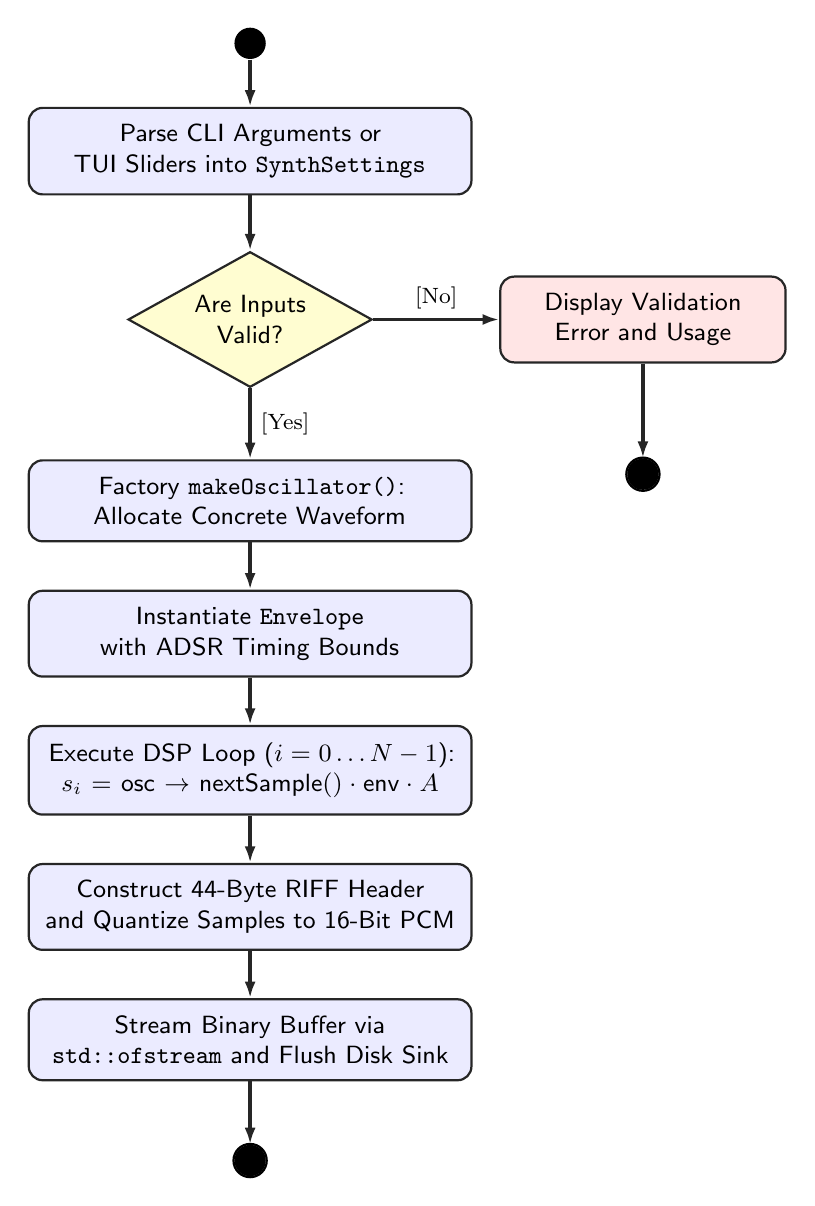
\begin{tikzpicture}[
    font=\small\sffamily,
    action/.style={
        draw=black!85,
        thick,
        fill=blue!8,
        rounded corners=5pt,
        align=center,
        inner sep=6pt,
        text width=5.2cm
    },
    decision/.style={
        draw=black!85,
        thick,
        fill=yellow!18,
        diamond,
        aspect=1.8,
        inner sep=3pt,
        align=center
    },
    flow/.style={
        very thick,
        -{Latex[length=6pt, width=4pt]},
        draw=black!85
    }
]

    % Nodes
    \node[circle, fill=black, inner sep=4pt] (start) at (0, 0) {};
    \node[action, below=0.6cm of start] (readInput) {Parse CLI Arguments or\\TUI Sliders into \texttt{SynthSettings}};
    \node[decision, below=0.7cm of readInput] (decVal) {Are Inputs\\Valid?};
    \node[action, fill=red!10, right=1.6cm of decVal, text width=3.2cm] (errMsg) {Display Validation\\Error and Usage};
    \node[circle, fill=black, inner sep=4pt, below=1.2cm of errMsg] (stopErrInner) {};
    \draw[thick] (stopErrInner) circle (6pt);

    \node[action, below=0.9cm of decVal] (factory) {Factory \texttt{makeOscillator()}:\\Allocate Concrete Waveform};
    \node[action, below=0.6cm of factory] (initEnv) {Instantiate \texttt{Envelope}\\with ADSR Timing Bounds};
    \node[action, below=0.6cm of initEnv] (dspLoop) {Execute DSP Loop ($i = 0 \dots N - 1$):\\$s_i = \text{osc}\to\text{nextSample}() \cdot \text{env} \cdot A$};
    \node[action, below=0.6cm of dspLoop] (riff) {Construct 44-Byte RIFF Header\\and Quantize Samples to 16-Bit PCM};
    \node[action, below=0.6cm of riff] (writeDisk) {Stream Binary Buffer via\\\texttt{std::ofstream} and Flush Disk Sink};
    \node[circle, fill=black, inner sep=4pt, below=0.8cm of writeDisk] (stopSuccessInner) {};
    \draw[thick] (stopSuccessInner) circle (6pt);

    % Flows
    \draw[flow] (start) -- (readInput);
    \draw[flow] (readInput) -- (decVal);
    \draw[flow] (decVal) -- node[above, font=\footnotesize] {[No]} (errMsg);
    \draw[flow] (errMsg) -- (stopErrInner);
    \draw[flow] (decVal) -- node[right, font=\footnotesize] {[Yes]} (factory);
    \draw[flow] (factory) -- (initEnv);
    \draw[flow] (initEnv) -- (dspLoop);
    \draw[flow] (dspLoop) -- (riff);
    \draw[flow] (riff) -- (writeDisk);
    \draw[flow] (writeDisk) -- (stopSuccessInner);

\end{tikzpicture}
}
\caption{UML Activity Diagram: Control flow highlighting input validation, sample generation loop, and binary output.}
\label{fig:uml_activity}
\end{figure}

% ---------------------------------------------------------------------
% RAW BINARY SERIALIZATION CODE
% ---------------------------------------------------------------------
Listing~\ref{lst:wavwriter_cpp} documents the low-level binary serialization implementation. The static method quantizes floating-point samples to 16-bit signed integers ($[-32768, 32767]$) and formats the canonical 44-byte RIFF/WAVE header directly into an unbuffered binary \texttt{std::ofstream}.

\begin{lstlisting}[language=C++, caption={Raw Binary RIFF/WAVE File Serializer (\texttt{src/WavWriter.cpp})}, label={lst:wavwriter_cpp}]
#include "WavWriter.h"
#include <algorithm>
#include <cmath>
#include <fstream>

std::int16_t WavWriter::toInt16(double sample) {
    sample = std::clamp(sample, -1.0, 1.0);
    return static_cast<std::int16_t>(std::lround(sample * 32767.0));
}

void WavWriter::writeU16(std::ostream& out, std::uint16_t value) {
    const char bytes[2] = {
        static_cast<char>(value & 0xFF),
        static_cast<char>((value >> 8) & 0xFF)
    };
    out.write(bytes, 2);
}

void WavWriter::writeU32(std::ostream& out, std::uint32_t value) {
    const char bytes[4] = {
        static_cast<char>(value & 0xFF),
        static_cast<char>((value >> 8) & 0xFF),
        static_cast<char>((value >> 16) & 0xFF),
        static_cast<char>((value >> 24) & 0xFF)
    };
    out.write(bytes, 4);
}

bool WavWriter::write(const std::string& filename,
                      const std::vector<double>& samples,
                      std::uint32_t sampleRate,
                      std::uint16_t channels) {
    std::ofstream file(filename, std::ios::binary);
    if (!file) return false;

    const std::uint16_t bitsPerSample = 16;
    const std::uint16_t blockAlign = channels * bitsPerSample / 8;
    const std::uint32_t byteRate = sampleRate * blockAlign;
    const std::uint32_t dataSize = static_cast<std::uint32_t>(samples.size() * 2);
    const std::uint32_t chunkSize = 36 + dataSize;

    // 1. RIFF Container Header
    file.write("RIFF", 4);
    writeU32(file, chunkSize);
    file.write("WAVE", 4);

    // 2. Format Chunk ("fmt ")
    file.write("fmt ", 4);
    writeU32(file, 16);               // Subchunk1Size (16 for PCM)
    writeU16(file, 1);                // AudioFormat (1 = PCM uncompressed)
    writeU16(file, channels);         // NumChannels (1 = Mono)
    writeU32(file, sampleRate);       // SampleRate (e.g. 44100 Hz)
    writeU32(file, byteRate);         // ByteRate
    writeU16(file, blockAlign);       // BlockAlign
    writeU16(file, bitsPerSample);    // BitsPerSample (16 bits)

    // 3. Data Chunk ("data")
    file.write("data", 4);
    writeU32(file, dataSize);

    // 4. Quantized PCM Little-Endian Sample Streaming
    std::vector<char> buffer(samples.size() * 2);
    for (std::size_t i = 0; i < samples.size(); ++i) {
        const std::uint16_t v = static_cast<std::uint16_t>(toInt16(samples[i]));
        buffer[2 * i]     = static_cast<char>(v & 0xFF);
        buffer[2 * i + 1] = static_cast<char>((v >> 8) & 0xFF);
    }
    file.write(buffer.data(), static_cast<std::streamsize>(buffer.size()));

    file.close();
    return !file.fail();
}
\end{lstlisting}

\clearpage
The generated output files were validated by inspecting the binary RIFF/WAVE header directly. Listing~\ref{lst:hex_dump} shows the hexadecimal dump of the generated file, confirming canonical 44-byte structure:

\begin{lstlisting}[language={}, caption={Binary Hexadecimal Dump of 44-Byte RIFF/WAVE Header}, label={lst:hex_dump}, basicstyle=\ttfamily\scriptsize, frame=single, rulecolor=\color{black!30}, backgroundcolor=\color{black!2}, numbers=none]
Offset    00 01 02 03 04 05 06 07  08 09 0A 0B 0C 0D 0E 0F   ASCII
----------------------------------------------------------------------
00000000  52 49 46 46 d8 5d 03 00  57 41 56 45 66 6d 74 20  |RIFF.]..WAVEfmt |
00000010  10 00 00 00 01 00 01 00  44 ac 00 00 88 58 01 00  |........D....X..|
00000020  02 00 10 00 64 61 74 61  b4 5d 03 00 00 00 a3 06  |....data.]......|
00000030  3a 0d b7 13 0c 1a 2a 20  03 26 89 2b db 2f db 33  |:.....* .&.+./.3|
\end{lstlisting}

The physical file size was verified against theoretical calculations:
\begin{align}
\text{File Size} &= 44 + \left(\text{Duration} \times f_s \times \text{Channels} \times \frac{\text{Bits}}{8}\right) \nonumber \\
&= 44 + (2.5 \times 44{,}100 \times 1 \times 2) = 220{,}544\text{ bytes}
\end{align}
The physical file created on disk matches $220{,}544$ bytes exactly.

\end{document}
